\section{Execution metadata}

\begin{frame}
 \begin{itemize}
  \item Problem: monitoring the execution of batch jobs
  \item Solution: letting Spring Batch storing execution metadata in a database
 \end{itemize}
\end{frame}

\begin{frame}
 \frametitle{Why storing execution metadata?}
 \begin{itemize}
  \item Spring Batch keeps track of batch execution
  \item Enables:
  \begin{itemize}
    \item Monitoring by querying metadata tables
    \item Restarting after a failure
  \end{itemize}
 \end{itemize}
\end{frame}


\begin{frame}
 \frametitle{Job, job instance, and job execution}
 \begin{figure}
  \begin{center}
  \includegraphics[width=10cm]{figures/jobinstance.pdf}
  \end{center}
 \end{figure}
\end{frame}


\begin{frame}
\frametitle{Job instance}
\begin{itemize}
 \item How to define a job instance?
 \item Thanks to job parameters
 \item Job parameters define the identity of the job instance
\end{itemize}
\end{frame}

\begin{frame}
\frametitle{Where is the metadata stored?}
\begin{itemize}
 \item Metadata are stored in a database 
 \begin{itemize}
  \item In-memory implementation for test/development
 \end{itemize}
 \item Monitoring tools can query metadata tables
\end{itemize}
\end{frame}

\begin{frame}
 \frametitle{Going further...}
 \begin{itemize}
  \item Spring Batch Admin, the web console for Spring Batch
  \item \code{JobExplorer} and \code{JobOperator} interfaces
  \item Spring JMX support
 \end{itemize}
\end{frame}

